% Compile with: pdflatex nq_frequency_replacement_part2_draft5.tex  (run twice for frame totals)
% Reading edition: 11 core frames, five interleaved explanatory supplements, and Backup A.
% Draft 4 merges frames 4, 7, 8 (as 8), 10 and 11 of a second agent's deck (nq_constrained_estimation_part2_draft.tex) into this one.
% Same preamble, colors, and fonts as Part 1. All figures are TikZ; no external images.
% Presenter notes are embedded in the source and hidden in the PDF.
\documentclass[aspectratio=169,11pt]{beamer}
% Same fonts as Part 1 when Latin Modern is installed; falls back to Computer Modern otherwise.
\IfFileExists{lmodern.sty}{\usepackage[T1]{fontenc}\usepackage{lmodern}}{}
\usepackage{amsmath,amssymb,booktabs,tabularx,colortbl}
\usepackage{tikz}
\usetikzlibrary{arrows.meta,positioning,calc}
\usefonttheme{professionalfonts}
\definecolor{Ink}{HTML}{182C42}
\definecolor{Accent}{HTML}{087F8C}
\definecolor{Muted}{HTML}{526474}
\definecolor{Pale}{HTML}{E6F2F3}
\definecolor{Warm}{HTML}{B8562E}
\setbeamercolor{normal text}{fg=Ink,bg=white}
\setbeamercolor{frametitle}{fg=Ink}
\setbeamercolor{title}{fg=Ink}
\setbeamercolor{structure}{fg=Accent}
\setbeamercolor{alerted text}{fg=Accent}
\setbeamerfont{frametitle}{size=\Large,series=\bfseries}
\setbeamerfont{title}{size=\LARGE,series=\bfseries}
\setbeamersize{text margin left=9mm,text margin right=9mm}
\setbeamertemplate{navigation symbols}{}
\setbeamertemplate{headline}{}
\setbeamertemplate{frametitle}{\vspace{3mm}\insertframetitle\par\vspace{1mm}}
\setbeamertemplate{footline}{%
  \hspace{9mm}{\color{Muted}\scriptsize Fixed-composition fitting\hfill Part 2\hspace{5mm}\insertframenumber\,/\,\inserttotalframenumber}\hspace{9mm}\vspace{3mm}}
\setbeamertemplate{itemize item}{\small\textbullet}
\setlength{\parskip}{0.35em}
\newcommand{\pis}{\pi^{\ast}}
\newcommand{\src}[1]{{\scriptsize\color{Muted}#1\par}}
\title{Fitting \texorpdfstring{$Q$}{Q} at a fixed composition}
\author{Peter Goodman}
\institute{Masel Lab}
\date{}
\pdfstringdefDisableCommands{\def\translate#1{#1}}

\tikzset{
  box/.style={draw=Ink,line width=0.5pt,rounded corners=1.2pt,fill=white,align=center,inner sep=2.5pt,font=\scriptsize},
  hi/.style={draw=Accent,line width=1.1pt,fill=Pale},
  arr/.style={-{Stealth[length=1.8mm]},line width=0.5pt,draw=Ink},
  lbl/.style={font=\scriptsize,text=Muted},
}

\begin{document}

% ---------------------------------------------------------------- Title
\begin{frame}[plain]
\vspace{5mm}
{\color{Accent}\small\bfseries PART 2\par}
\vspace{5mm}
{\usebeamerfont{title}\inserttitle\par}
\vspace{7mm}

\vspace{12mm}
{\insertauthor\quad\textcolor{Muted}{\insertinstitute}\par}
\note{Part 1 showed that frequency replacement with fixed off-diagonal factors is exact only for reversible models. Part 2 explains the alternative: fix the composition first and fit only the generators that have it as equilibrium, and what that requires inside nQMaker. Part 3 covers the concrete code changes and testing.}
\end{frame}

% ---------------------------------------------------------------- 1. The reversible workflow and the proposed solution
\begin{frame}{The reversible workflow we want to reproduce}
\small
\textbf{Wheeler et al.\ 2026.}\quad Models trained on filtered MSAs give better gene trees, but filtering
removes residues unevenly, so the fitted $\pi_{\mathrm{clean}}$ drifts from the composition of the data
the model is applied to. \textbf{Remedy:} exchangeabilities from the filtered MSAs, composition from the target data,
\[
 q_{ij}=R^{\mathrm{clean}}_{ij}\,\pi^{\mathrm{target}}_{j}\quad(i\ne j),
 \qquad\text{exact since $R=R^{\mathsf T}$ (Part 1): }\ \pi_iq_{ij}=\pi_jq_{ji}\ \forall\,\pi .
\]
\textbf{The same move for a nonreversible fit fails.}\quad Split $Q^{\mathrm{clean}}$ into factors and a composition, then swap:
\[
 A_{ij}=\frac{q^{\mathrm{clean}}_{ij}}{\pi_{\mathrm{clean},j}},\qquad
 \widetilde q_{ij}=A_{ij}\,\pi^{\mathrm{target}}_j,
 \qquad
 (\pi^{\mathrm{target}}\widetilde Q)_j=\pi^{\mathrm{target}}_j\sum_{i\ne j}\pi^{\mathrm{target}}_i\,(A_{ij}-A_{ji}) .
\]
The residual vanishes for every target only if $A=A^{\mathsf T}$, which is reversibility of $Q^{\mathrm{clean}}$.

\vspace{1mm}
\alert{\textbf{Proposed solution:} constrained optimization. First determine the target composition $\pis$;
then fit $Q$ on the filtered training data subject to $\pis Q=0$. $\pis$ is an input of the fit, not an output.}
\vspace{2mm}
\note{Wheeler et al. (bioRxiv 10.64898/2025.12.01.691663) trained on 1000 OrthoMaM loci and tested on 5769; Divvier-pf was the best training filter. Their Methods take the composition from the testing data set, which in some cases was itself mildly filtered. For this project Peter specifies the uncleaned alignments as the target source. The residual formula is the Part 1 stationarity identity. For the nonreversible case no fixed factor permits arbitrary replacement, so the replacement step has to become a constraint on the fit itself.}
\end{frame}

% ---------------------------------------------------------------- 2. Counting dimensions
\begin{frame}{The admissible set at a fixed composition}
\small
With $\pis$ fixed, stationarity is \emph{linear} in the off-diagonal rates:
\[
 (\pis Q)_j=\sum_{i\ne j}\pi^{\ast}_i q_{ij}-\pi^{\ast}_j\sum_{k\ne j}q_{jk}=0,
 \qquad j=1,\ldots,20 .
\]
The 20 residuals sum to zero: \textbf{19 independent equations}. Scale fix: $-\sum_i\pi^{\ast}_i q_{ii}=1$.

\begin{center}
\renewcommand{\arraystretch}{1.2}
\begin{tabular}{@{}l@{\hspace{7mm}}r@{\hspace{7mm}}r@{}}
\toprule
\textbf{Positive generators $Q$} & \textbf{Raw} & \textbf{Scale removed}\\
\midrule
Unrestricted (nQMaker today; $\pi$ solved from $Q$) & 380 & 379\\
Stationary at the specified $\pis$\quad ($\mathcal G_{\pis}$) & 361 & 360\\
Reversible and stationary at $\pis$ & 190 & 189\\
\bottomrule
\end{tabular}
\end{center}

\alert{$\boldsymbol{\mathcal G_{\pis}}$ is a flat convex slice, and every reversible $Q$ with equilibrium $\pis$ lies inside it.}
\note{This promotes the Part 1 backup table. The point to land: at a fixed target the constraint is a set of linear equations in the rates, so the admissible set is a flat slice of the positive orthant, and the reversible fit at the same target is a point inside the slice, which is why it can serve as a start and a nested control. Dimension is a parameter count, not a statement about identifiability.}
\end{frame}

% ---------------------------------------------------------------- 3. Visualization (from presentation 2)
\begin{frame}{A smaller family, still allowing nonreversibility}
\begin{columns}[c,onlytextwidth]
\column{.55\textwidth}
\centering
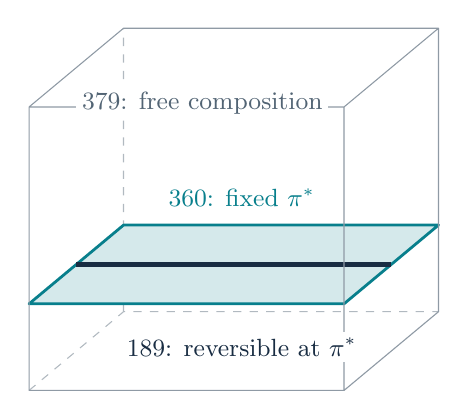
\begin{tikzpicture}[x=1cm,y=1cm,line join=round]
\coordinate (A) at (0,0); \coordinate (B) at (4,0);
\coordinate (C) at (5.2,1); \coordinate (D) at (1.2,1);
\coordinate (E) at (0,3.6); \coordinate (F) at (4,3.6);
\coordinate (G) at (5.2,4.6); \coordinate (H) at (1.2,4.6);
\draw[Muted!45,dashed] (A)--(D)--(C) (D)--(H);
\filldraw[fill=Accent!17,draw=Accent,line width=1pt] (0,1.1)--(4,1.1)--(5.2,2.1)--(1.2,2.1)--cycle;
\draw[Ink,line width=1.6pt] (.6,1.6)--(4.6,1.6);
\draw[Muted!65] (A)--(B)--(C)--(G)--(H)--(E)--cycle (E)--(F)--(G) (B)--(F);
\node[fill=white,inner sep=2pt,text=Muted,font=\small] at (2.2,3.65) {379: free composition};
\node[fill=white,inner sep=2pt,text=Accent,font=\small] at (2.7,2.45) {360: fixed $\pis$};
\node[fill=white,inner sep=2pt,text=Ink,font=\small] at (2.7,.55) {189: reversible at $\pis$};
\end{tikzpicture}
\column{.41\textwidth}
\raggedright
\textbf{Every fitted matrix must satisfy}
\[
 q_{ij}>0\ (i\ne j),\quad Q\mathbf1=0,
\]
\[
 \pis Q=0,\qquad -\sum_i\pi_i^{\ast} q_{ii}=1.
\]
\vspace{3mm}
\alert{The optimizer can leave the reversible family while keeping $\pis$ fixed.}
\end{columns}
\vfill
{\small\color{Muted}Schematic only: dimensions and geometry are compressed. The fixed-target family is an affine slice with positivity constraints.\par}
\note{The enclosing cube is a conceptual container for normalized positive generators, not literal coordinate axes. At a fixed target, stationarity and mean-rate normalization are linear constraints on the 380 off-diagonals, so their positive intersection is a convex, relatively open affine slice of dimension 360. The reversible subfamily has dimension 189 and is contained in it. The line is a dimensional cartoon only.}
\end{frame}


% Reading supplement after original slide 4.
\begingroup
\setbeamertemplate{footline}{%
  \hspace{9mm}{\color{Muted}\scriptsize EXPLANATORY BACKUP\quad Explains the fixed-target model space\hfill\insertframenumber\,/\,\inserttotalframenumber}\hspace{9mm}\vspace{3mm}}
\begin{frame}{Supplement: why search the blue plane?}
\begin{columns}[c,onlytextwidth]
\column{.51\textwidth}
\centering
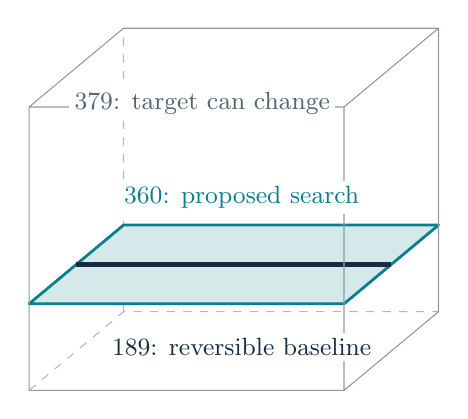
\begin{tikzpicture}[x=1cm,y=1cm,line join=round]
\coordinate (A) at (0,0); \coordinate (B) at (4,0);
\coordinate (C) at (5.2,1); \coordinate (D) at (1.2,1);
\coordinate (E) at (0,3.6); \coordinate (F) at (4,3.6);
\coordinate (G) at (5.2,4.6); \coordinate (H) at (1.2,4.6);
\draw[Muted!45,dashed] (A)--(D)--(C) (D)--(H);
\filldraw[fill=Accent!17,draw=Accent,line width=1pt] (0,1.1)--(4,1.1)--(5.2,2.1)--(1.2,2.1)--cycle;
\draw[Ink,line width=1.6pt] (.6,1.6)--(4.6,1.6);
\draw[Muted!65] (A)--(B)--(C)--(G)--(H)--(E)--cycle (E)--(F)--(G) (B)--(F);
\node[fill=white,inner sep=2pt,text=Muted,font=\small] at (2.2,3.65) {379: target can change};
\node[fill=white,inner sep=2pt,text=Accent,font=\small] at (2.7,2.45) {360: proposed search};
\node[fill=white,inner sep=2pt,text=Ink,font=\small] at (2.7,.55) {189: reversible baseline};
\end{tikzpicture}
\column{.47\textwidth}
\small
\textbf{The target is already an input.} Estimate $\pis$ from the uncleaned alignments. Fit $Q$ to the cleaned alignments while keeping $\pis Q=0$.

\textbf{Black line: reversible family.} The frequency-corrected matrices in the earlier workflow lie here after normalization.

\textbf{Blue plane: proposed family.} Search all 360 dimensions of $\mathcal G_{\pis}$, including 171 dimensions beyond reversibility.

\alert{How much can the added freedom improve the fit and downstream inference?}
\end{columns}
\vfill
{\footnotesize\color{Muted}Schematic. The earlier fit-then-swap workflow is not the same as refitting at the target. The larger family contains the reversible baseline, but better inference requires testing.}
\end{frame}
\endgroup

% ---------------------------------------------------------------- 4. nQMaker today
\begin{frame}{nQMaker today (Dang et al.\ 2022)}
\begin{center}
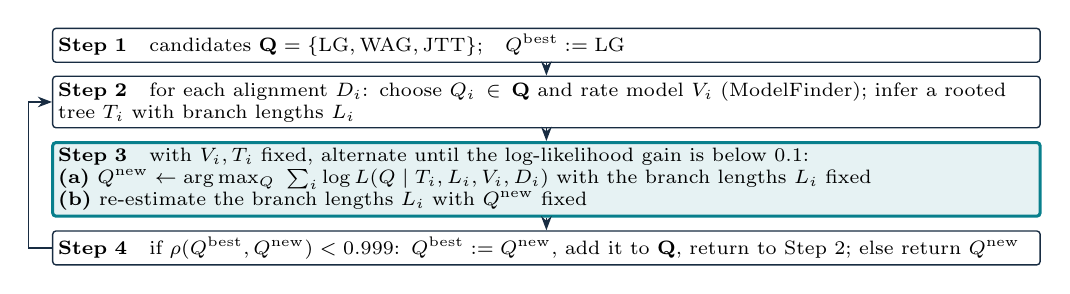
\begin{tikzpicture}[node distance=1.6mm and 5mm]
 \node[box,text width=124mm,align=left,inner sep=2pt] (s1) {\textbf{Step 1}\quad candidates $\mathbf Q=\{\mathrm{LG},\mathrm{WAG},\mathrm{JTT}\}$;\quad $Q^{\mathrm{best}}:=\mathrm{LG}$};
 \node[box,text width=124mm,align=left,inner sep=2pt,below=of s1] (s2) {\textbf{Step 2}\quad for each alignment $D_i$: choose $Q_i\in\mathbf Q$ and rate model $V_i$ (ModelFinder); infer a rooted tree $T_i$ with branch lengths $L_i$};
 \node[box,hi,text width=124mm,align=left,inner sep=2pt,below=of s2] (s3) {\textbf{Step 3}\quad with $V_i,T_i$ fixed, alternate until the log-likelihood gain is below $0.1$:\\
   \textbf{(a)} $Q^{\mathrm{new}}\leftarrow\arg\max_Q\ \sum_i\log L(Q\mid T_i,L_i,V_i,D_i)$ with the branch lengths $L_i$ fixed\\
   \textbf{(b)} re-estimate the branch lengths $L_i$ with $Q^{\mathrm{new}}$ fixed};
 \node[box,text width=124mm,align=left,inner sep=2pt,below=of s3] (s4) {\textbf{Step 4}\quad if $\rho(Q^{\mathrm{best}},Q^{\mathrm{new}})<0.999$: $Q^{\mathrm{best}}:=Q^{\mathrm{new}}$, add it to $\mathbf Q$, return to Step 2;\ else return $Q^{\mathrm{new}}$};
 \draw[arr] (s1)--(s2); \draw[arr] (s2)--(s3); \draw[arr] (s3)--(s4);
 \draw[arr] (s4.west) -- ++(-3mm,0) |- (s2.west);
\end{tikzpicture}
\end{center}
\vspace{-1mm}
{\small
\textbf{Each trial $Q$ (3a).}\quad Rates $\to Q\to$ \alert{solve $\pi$ from $Q$} $\to$ rescale to mean rate 1 $\to$ score
$\displaystyle \ell(Q)=\sum_i\log L\big(Q\mid T_i,L_i,V_i,D_i\big)$, with trees, branch lengths and rate models held fixed.\par}
\vspace{1mm}
\alert{\textbf{Proposal:} Reuse the likelihood calculation, but change how trial matrices are built.}
\note{Redrawn from Figure 1 and the numbered list on pp. 1112 to 1113 of the nQMaker paper, read in full. Commands in the paper: iqtree2 -S ALN_DIR -mset LG,WAG,JTT -cmax 4 for steps 1 and 2, and iqtree2 -S ALN_DIR.best_model.nex -te ALN_DIR.treefile --model-joint NONREV+FO for step 3. Source facts at IQ-TREE 3 commit 63c330d9: the optimizer variables in 3a are 379 of the 380 raw off-diagonal rates (one is never handed to the optimizer, which pins the overall scale), each inside the default box MIN_RATE 1e-4 to MAX_RATE 100; each trial rebuilds Q, solves state_freq from Q, and rescales so the expected rate is 1 (ModelMarkov::decomposeRateMatrixNonrev); BFGS with forward finite differences. The likelihood is the ordinary sum over alignments of pattern-weighted log-likelihoods, nQMaker Equation 4. In the source the linked update also lets continuous site-rate parameters move.}
\end{frame}

% ---------------------------------------------------------------- 5. Change map
\begin{frame}{What changes and what does not}
\begin{center}
\renewcommand{\arraystretch}{1.25}
\small
\begin{tabularx}{\textwidth}{@{}p{0.12\textwidth}p{0.31\textwidth}X@{}}
\toprule
\textbf{nQMaker} & \textbf{Today} & \textbf{Fixed-composition version}\\
\midrule
Step 1 & LG, WAG, JTT with their own $\pi$ & \emph{proposed:} same exchangeabilities rebuilt at $\pis$, $q_{ij}=R_{ij}\pi^{\ast}_j$\\
Step 2 & ModelFinder, rooted trees & unchanged\\
\rowcolor{Pale}
Step 3a & 379 rates; $\pi$ solved from $Q$ at each trial & \textbf{360 coordinates; $\pis$ held fixed; every trial $Q$ is built so that $\pis Q=0$}\\
Step 3b & branch lengths, $Q$ fixed & unchanged\\
Step 4 & add $Q^{\mathrm{best}}$ to the candidates & unchanged; the added matrix is a fixed candidate\\
\bottomrule
\end{tabularx}
\end{center}
\vspace{2mm}
\alert{How do we make sure that the optimizer in step 3a only produces $Q\in\mathcal G_{\pis}$, so that we can use
the same likelihood architecture?}
\note{The likelihood engine, transition matrices, pruning, branch-length and rate optimizers are reused as they are. The single substantive change is the map from optimizer variables to Q in step 3a. Peripheral changes are the target as an input, the seed, the parameter count, and output. The Step 1 rebuild is a protocol choice: candidates only select per-alignment models and guide trees, so the constrained fit is valid either way; rebuilding keeps every stage on the same composition convention.}
\end{frame}


% Reading supplements between original slides 6 and 7.
\begingroup
\setbeamertemplate{footline}{%
  \hspace{9mm}{\color{Muted}\scriptsize EXPLANATORY BACKUP\quad Explains how the jump chain relates to $Q$\hfill\insertframenumber\,/\,\inserttotalframenumber}\hspace{9mm}\vspace{3mm}}
\begin{frame}{Supplement: waiting times and destinations}
\small
A continuous-time Markov chain stays in one amino acid for a random time,
then jumps to another. $Q$ contains both parts of this description.

\vspace{2mm}
\begin{columns}[T,onlytextwidth]
\column{.48\textwidth}
\textbf{When does the next change occur?}
\[
 \lambda_i=\sum_{j\ne i}q_{ij}=-q_{ii}.
\]
The waiting time in state $i$ is exponential:
\[
 T_i\sim\operatorname{Exp}(\lambda_i),\qquad
 \mathbb E[T_i]=1/\lambda_i.
\]
A larger exit rate means a shorter average wait.
\column{.48\textwidth}
\textbf{Where does the process go next?}
\[
 K_{ij}=\frac{q_{ij}}{\lambda_i}\quad(i\ne j),\qquad K_{ii}=0.
\]
Conditional on leaving $i$, row $i$ of $K$ gives the probabilities of the next state.

The \textbf{embedded jump chain} records this sequence of states and omits the waiting times.
\end{columns}
\vspace{3mm}
\alert{Together, destinations and waiting times recover the same process:
$q_{ij}=\lambda_iK_{ij}$, $q_{ii}=-\lambda_i$.}
\end{frame}
\endgroup

\begingroup
\setbeamertemplate{footline}{%
  \hspace{9mm}{\color{Muted}\scriptsize EXPLANATORY BACKUP\quad Explains exit rates, jump probabilities, and $P(t)$\hfill\insertframenumber\,/\,\inserttotalframenumber}\hspace{9mm}\vspace{3mm}}
\begin{frame}{Supplement: one row of $Q$, worked through}
\small
\textbf{A three-state example.} Suppose the row for state A is
\[
 (q_{\mathrm{AA}},q_{\mathrm{AB}},q_{\mathrm{AC}})=(-5,\,2,\,3).
\]
\begin{center}
\renewcommand{\arraystretch}{1.25}
\begin{tabular}{@{}ll@{}}
\toprule
\textbf{Quantity} & \textbf{Meaning in this example}\\
\midrule
Exit rate $\lambda_{\mathrm A}=5$ & Total rate of leaving A\\
Mean wait $1/\lambda_{\mathrm A}=0.2$ & Average time spent in A per visit\\
$K_{\mathrm{AB}}=2/5$, $K_{\mathrm{AC}}=3/5$ & Next change goes to B or C with these probabilities\\
\bottomrule
\end{tabular}
\end{center}
\textbf{$K$ and $P(t)=e^{tQ}$ answer different questions.}

$K_{\mathrm{AB}}$: given that A changes, is B the \emph{next} state?\\
$P_{\mathrm{AB}}(t)$: starting at A, are we in B after elapsed time $t$?

\alert{$P(t)$ accounts for any number of jumps, including a return to A.
Thus $K_{ii}=0$, while $P_{ii}(t)$ can be positive.}
\end{frame}
\endgroup



% ---------------------------------------------------------------- 6. Jump chain builds Q (from presentation 2)
\begin{frame}{A jump chain builds a target-stationary $Q$}
\small\setlength{\parskip}{0.25em}
\textbf{Choose destinations.}\quad $K_{ij}$ is the probability of jumping from $i$ to $j$:
\[
 K_{ii}=0,\qquad K_{ij}>0\ (i\ne j),\qquad \sum_j K_{ij}=1.
\]
\textbf{Solve once per trial.}\quad Find jump-event frequencies $\nu$:
\[
 \nu K=\nu,\qquad \sum_i\nu_i=1.
\]
\textbf{Set waiting times.}\quad Exit rate $\lambda_i=\nu_i/\pi_i^{\ast}$ gives
\[
 q_{ij}=\lambda_iK_{ij}\ (i\ne j),\qquad q_{ii}=-\lambda_i.
\]
\vspace{-1mm}
\[
 (\pis Q)_j=\underbrace{\sum_{i\ne j}\nu_i K_{ij}}_{\text{inflow}}-\underbrace{\nu_j}_{\text{outflow}}=0,
 \qquad -\sum_i\pi_i^{\ast} q_{ii}=\sum_i\nu_i=1.
\]
\alert{Every such $K$ builds a feasible, normalized $Q$. Distinct $K$ give distinct $Q$, since $K_{ij}=q_{ij}/(-q_{ii})$.}
\note{K is the embedded jump chain, distinct from the finite-time P(t) = exp(tQ). In state i the holding time is exponential with mean 1/lambda_i = pi-star_i/nu_i. nu is the long-run fraction of jump events leaving each state; pi-star is the fraction of elapsed time. Inflow to j is sum over i of pi-star_i q_ij = sum nu_i K_ij; outflow is pi-star_j times the total leaving rate lambda_j, which equals nu_j. Positive off-diagonals give irreducibility and a unique positive nu: one normalized linear solve, the same size as today's solve of pi from Q. What this slide proves is that the map from K to Q lands inside G at pi-star, positive, zero row sums, stationary, unit mean rate; injectivity is the one-line remark that K can be read back from Q. Surjectivity is the next slide.}
\end{frame}

% ---------------------------------------------------------------- 7. Surjectivity (from presentation 2 backup A)
\begin{frame}{Every feasible positive $Q$ has unique coordinates}
Given $Q$ with $\pis Q=0$ and $-\sum_i\pi_i^{\ast} q_{ii}=1$, recover
\[
 \lambda_i=-q_{ii},\qquad
 K_{ij}=\frac{q_{ij}}{\lambda_i}\ (i\ne j),\qquad K_{ii}=0,
 \qquad \nu_i=\pi_i^{\ast}\lambda_i.
\]
Then $\sum_i\nu_i=1$ and, for each $j$,
\[
 (\nu K)_j=\sum_{i\ne j}\pi_i^{\ast} q_{ij}
 =-\pi_j^{\ast} q_{jj}=\nu_j.
\]
The builder recovers $q_{ij}=(\nu_i/\pi_i^{\ast})K_{ij}$ exactly.
For a fixed reference destination $r(i)\ne i$, the log-ratios are
\[
 z_{ij}=\log\!\left(\frac{K_{ij}}{K_{i,r(i)}}\right).
\]
\alert{Every feasible positive $Q$ is reached once: a bijection with $\mathbb R^{360}$.}
\vfill
\src{Assumes positive off-diagonals and target. Actual finite coordinate bounds restrict the represented family.}
\note{The inverse establishes coverage of all strictly positive normalized target-stationary matrices, including reversible ones, so nothing in G at pi-star is out of reach of the optimizer. sum nu_i = 1 is exactly the unit mean-rate condition; nu K = nu is exactly pi-star Q = 0 rewritten. This says nothing by itself about sample identifiability or global likelihood attainment.}
\end{frame}

% ---------------------------------------------------------------- 8. What the optimizer proposes: today versus log-ratios
\begin{frame}{Optimizer proposals: nQMaker today versus log-ratios}
\small
\begin{columns}[T,onlytextwidth]
\column{.44\textwidth}
\centering
\textbf{nQMaker today: 379 raw rates}\par
\vspace{2mm}
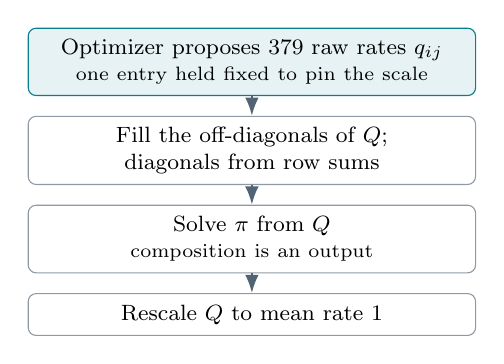
\begin{tikzpicture}[x=1cm,y=1cm,>=Latex,
 box/.style={draw=Muted!65,rounded corners=1mm,align=center,inner sep=4pt,font=\footnotesize,text width=5.4cm},
 arr/.style={->,draw=Muted,line width=.8pt}]
\node[box,draw=Accent,fill=Pale] (a) at (0,0) {Optimizer proposes 379 raw rates $q_{ij}$\\{\scriptsize one entry held fixed to pin the scale}};
\node[box,below=2.5mm of a] (b) {Fill the off-diagonals of $Q$;\\diagonals from row sums};
\node[box,below=2.5mm of b] (c) {Solve $\pi$ from $Q$\\{\scriptsize composition is an output}};
\node[box,below=2.5mm of c] (d) {Rescale $Q$ to mean rate 1};
\draw[arr] (a)--(b); \draw[arr] (b)--(c); \draw[arr] (c)--(d);
\end{tikzpicture}
\par\vspace{1.5mm}
{\footnotesize\color{Muted}Each raw rate kept inside $[10^{-4},100]$; no per-row reference.\par}
\column{.04\textwidth}
\centering
\rule{0.4pt}{58mm}
\column{.50\textwidth}
\raggedright
\textbf{Proposed: 18 log-ratios per row}\par
\vspace{2mm}
For amino acid $i$, choose one fixed reference destination $r(i)\ne i$.
\[
 z_{ij}=\log\!\left(\frac{K_{ij}}{K_{i,r(i)}}\right),\qquad z_{i,r(i)}=0.
\]
\textbf{Interpretation.}\quad $z_{ij}=\log 2$ makes destination $j$ twice as likely as the reference.
\vspace{1mm}
\[
 \underbrace{(0,\log 2,\log 4)}_{\text{log-ratios}}\ \longmapsto\ \underbrace{(1,2,4)}_{\text{weights}}\ \longmapsto\ \underbrace{\left(\tfrac17,\tfrac27,\tfrac47\right)}_{\text{row of }K}
\]
{\footnotesize\color{Muted}illustration with three destinations; $K$ then feeds the jump-chain build.\par}
\end{columns}
\note{Left column verified in IQ-TREE 3 source at commit 63c330d9: NONREV keeps 380 raw off-diagonal rates row-major; setVariables hands the first 379 to the optimizer, so the last stored entry (row V, column Y) is the single globally pinned value; setBounds puts MIN_RATE and MAX_RATE on each optimized rate; decomposeRateMatrixNonrev fills Q, solves state_freq from Q, and rescales to mean rate 1. There is no per-row normalization or reference in NONREV. Right column: the reference logit of zero removes the redundant common shift of a row's 19 logits; it fixes a ratio convention, not a physical rate. References stay fixed across iterations and linked partitions; the default is the row maximum of the target-rebuilt LG seed. Use a stable softmax when exponentiating.}
\end{frame}


% Reading recaps after original slide 9.
\begingroup
\setbeamertemplate{footline}{%
  \hspace{9mm}{\color{Muted}\scriptsize EXPLANATORY BACKUP\quad Explains the proposed construction in plain language\hfill\insertframenumber\,/\,\inserttotalframenumber}\hspace{9mm}\vspace{3mm}}
\begin{frame}{Supplement: how we build each trial matrix}
\textbf{The problem.} An ordinary nonreversible trial matrix determines its own equilibrium.
Our trial matrix must instead have the prescribed equilibrium $\pis$.

\vspace{1mm}
\begin{enumerate}
\item \textbf{Propose destination preferences.} Convert 360 optimizer coordinates into the rows of a valid jump matrix $K$.
\item \textbf{Work out visit frequencies.} Solve $\nu K=\nu$ once for this trial.
\item \textbf{Fill in the waiting times.} Set $\tau_i=\pi_i^\ast/\nu_i$.
These waits make the fraction of time in each state equal to the target.
\item \textbf{Build and score $Q$.} Use $q_{ij}=K_{ij}/\tau_i$ and $q_{ii}=-1/\tau_i$, then evaluate the ordinary phylogenetic likelihood.
\end{enumerate}
\vspace{1mm}
\alert{The optimizer changes the destination preferences. The builder computes
the waiting times required by the fixed target.}


\end{frame}
\endgroup

\begingroup
\setbeamertemplate{footline}{%
  \hspace{9mm}{\color{Muted}\scriptsize EXPLANATORY BACKUP\quad Explains the optimizer coordinates\hfill\insertframenumber\,/\,\inserttotalframenumber}\hspace{9mm}\vspace{3mm}}
\begin{frame}{Supplement: why continuous log-ratios?}
\small
\textbf{Direct probabilities have coupled constraints.} Each row needs 19 positive probabilities
summing to one. Independent changes can break that sum or make an entry negative.

\textbf{Log-ratios provide 18 free numbers per row.} Choose one fixed reference $r(i)\ne i$:
\[
 z_{ij}=\log\frac{K_{ij}}{K_{i,r(i)}},\qquad z_{i,r(i)}=0,
 \qquad K_{ij}=\frac{e^{z_{ij}}}{\sum_{k\ne i}e^{z_{ik}}}\quad(j\ne i).
\]
Every finite real proposal gives positive probabilities summing to one.
Fixing the reference removes the redundant common shift of a row's logits.

\textbf{These variables are continuous.} Small changes in $z$ produce smooth changes in $K$,
its stationary vector $\nu$, and $Q$, throughout the strictly positive family.
There are $20\times18=360$ free coordinates.

\textbf{Why start with logs?} An additive change adjusts a probability ratio multiplicatively.
Positive ratios are also continuous and remain a valid comparison option.

\vfill
\src{Implementation: stable softmax; scale-aware finite differences near $z=0$.
Finite bounds restrict coverage. Smoothness alone does not guarantee good conditioning or convergence.}
\end{frame}
\endgroup

% ---------------------------------------------------------------- 9. Likelihood evaluation, proposed versus current (from presentation 2 slide 9)
\begin{frame}{Comparison of likelihood evaluation inside step 3a}
\begin{center}
\resizebox{\textwidth}{!}{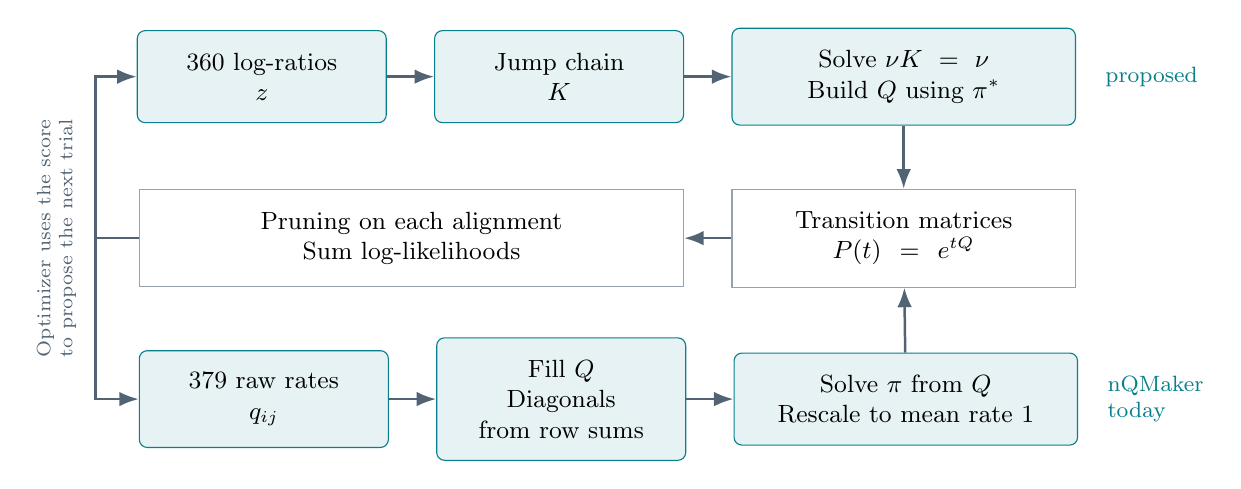
\begin{tikzpicture}[x=1cm,y=1cm,>=Latex,
 new/.style={draw=Accent,fill=Pale,rounded corners=1mm,align=center,inner sep=8pt,font=\small},
 old/.style={draw=Muted!60,align=center,inner sep=8pt,font=\small},
 arr/.style={->,draw=Muted,line width=.9pt}]
% proposed row
\node[new,text width=2.6cm] (z) at (0,0) {360 log-ratios\\$z$};
\node[new,text width=2.6cm,right=6mm of z] (k) {Jump chain\\$K$};
\node[new,text width=3.8cm,right=6mm of k] (q) {Solve $\nu K=\nu$\\Build $Q$ using $\pis$};
\draw[arr] (z)--(k); \draw[arr] (k)--(q);
\node[font=\footnotesize,text=Accent,anchor=west] at ($(q.east)+(.25,0)$) {proposed};
% shared likelihood row
\node[old,text width=3.8cm,below=8mm of q] (p) {Transition matrices\\$P(t)=e^{tQ}$};
\node[old,text width=6.35cm,anchor=east] (l) at ($(p.west)+(-.6,0)$) {Pruning on each alignment\\Sum log-likelihoods};
\draw[arr] (q)--(p); \draw[arr] (p)--(l);
% current nQMaker row
\node[new,text width=2.6cm,below=8mm of l.south west,anchor=north west] (r) {379 raw rates\\$q_{ij}$};
\node[new,text width=2.6cm,right=6mm of r] (f) {Fill $Q$\\Diagonals from row sums};
\node[new,text width=3.8cm,right=6mm of f] (s) {Solve $\pi$ from $Q$\\Rescale to mean rate 1};
\draw[arr] (r)--(f); \draw[arr] (f)--(s);
\draw[arr] (s)--(p);
\node[font=\footnotesize,text=Accent,anchor=west,align=left] at ($(s.east)+(.25,0)$) {nQMaker\\today};
% feedback from the score to both proposal rows
\coordinate (fb) at ($(l.west)+(-.55,0)$);
\draw[draw=Muted,line width=.9pt] (l.west)--(fb);
\draw[arr] (fb) |- (z.west);
\draw[arr] (fb) |- (r.west);
\node[font=\scriptsize,text=Muted,rotate=90,align=center,anchor=south] at ($(fb)+(-.12,0)$) {Optimizer uses the score\\to propose the next trial};
\end{tikzpicture}}
\end{center}
\note{Teal boxes: what the optimizer variables are and how a trial Q is built from them; white boxes: the likelihood machinery, identical for both. Top row is the proposal, bottom row is NONREV today. All nuisance quantities are fixed for this conditional evaluation: rooted topology, branch lengths, rate parameters. Stationary root weights are pi-star in the proposal and the solved pi today. The linear solve in the proposal, nu from K, replaces the solve of pi from Q, same size; equal runtime is plausible but not measured. Unrestricted log-ratios cover every positive normalized Q at pi-star; finite numerical bounds restrict that coverage, and feasibility does not guarantee a global optimum.}
\end{frame}

% ---------------------------------------------------------------- 10. Other changes (from presentation 2 slide 10)
\begin{frame}{Other changes to the nQMaker process}
\small
\renewcommand{\arraystretch}{1.08}
\begin{tabularx}{\textwidth}{@{}p{.22\textwidth}X@{}}
\toprule
\textbf{Where} & \textbf{Current proposal / remaining choice}\\
\midrule
Before training & Estimate one positive $\pis$ from the original training data. Hold it fixed across cleaning treatments.\\
Initial candidates & Rebuild LG/WAG/JTT using $q_{ij}\propto R_{ij}\pi_j^{\ast}$, with the per-alignment frequency variant \texttt{+F} switched off; target-rebuilt LG is the first fitting seed.\\
Throughout fitting & Keep root frequencies at $\pis$. Share one $Q$ across training genes; retain the declared nuisance updates.\\
Later rounds & The learned $Q$ re-enters step 2 as a fixed matrix, as LG does today: no per-alignment refit of coordinates or composition. IQ-TREE currently refuses mixed reversible and nonreversible candidate sets.\\
Final fit & Use two starts: target-rebuilt LG and the reversible fit \texttt{GTR20+F\{$\pis$\}} on the same training data. Keep the reversible fit as an incumbent. With the same objective and a numerical domain containing that start, the returned likelihood should be at least as high.\\
\bottomrule
\end{tabularx}
\note{Target-rebuilt guide matrices are the primary protocol, not a mathematical prerequisite to constrained fitting. ModelFinder's default protein frequency variants are the plain matrix and +F (empirical frequencies of that alignment), main/phylotesting.cpp line 205 at commit 63c330d9; +F would refit the composition per alignment. A user-defined matrix file is read with num_params = 0, so passing the learned Q as a file keeps it fixed. The mixed reversible/nonreversible guard is in main/phylotesting.cpp (mixRevNonrev). The two-starts item is about the nonconcave likelihood: the reversible fit at the target is a member of the constrained family, so the constrained optimum cannot legitimately fall below it; starting from it makes that check operational. Derivatives, parameter accounting, persistence and regression belong to Part 3.}
\end{frame}

% ---------------------------------------------------------------- Backup A: why log-ratios rather than the entries of K
\appendix
\setbeamertemplate{footline}{%
  \hspace{9mm}{\color{Muted}\scriptsize Fixed-composition fitting\hfill Backup A}\hspace{9mm}\vspace{3mm}}
\begin{frame}[noframenumbering]{Backup A: choosing coordinates for $K$}
\small
Row $i$ of $K$: 19 positive entries that sum to one, so 18 degrees of freedom. BFGS applies only per-coordinate box limits.

\textbf{What should the optimizer propose?}

\textbf{All 19 entries, renormalized inside the builder.}\quad
$K_{ij}=w_{ij}/\sum_k w_{ik}$. A common factor on the row changes nothing: one redundant direction.
Pinning one entry, $w_{i,r(i)}=c$, removes it. These are the \emph{positive weights}.

\textbf{18 entries, the last set to one minus their sum.}\quad
$K_{i,r(i)}=1-\sum_{j\ne r(i)}K_{ij}$ can go negative under independent proposals; box limits do not enforce the sum constraint.

\textbf{18 log-ratios.}\quad
$z_{ij}=\log(w_{ij}/c)\in\mathbb R$: the resulting weights are positive by construction.
\[
 \text{weights: } w_{ij}\mapsto w_{ij}+\delta,
 \qquad\qquad
 \text{log-ratios: } \frac{K_{ij}}{K_{i,r(i)}}\mapsto e^{\delta}\,\frac{K_{ij}}{K_{i,r(i)}} .
\]
An additive $\delta$ is large for a rare substitution and negligible for a common one; $e^{\delta}$ is the same relative change for both.


\vfill

\note{BFGS starts from an identity Hessian and treats every coordinate on the same absolute scale; in positive weights a rare substitution with w = 0.001 receives the same absolute step as a common one with w = 5. In toy comparisons in the synthesis, positive-weight runs stopped early after failed line searches in 3 of 4 instances while log runs reached the gradient tolerance; that is evidence for a starting choice, not a theorem; the numbers are in the unified discrepancy synthesis, Section 10.}
\end{frame}

\end{document}
